% =====================================================================================
%  CVPR 2027 submission (anonymous review version)
%  BUILD: put this file, refs.bib and figures/ into the OFFICIAL CVPR 2027 author kit
%  (https://github.com/cvpr-org/author-kit: cvpr.sty, ieeenat_fullname.bst). Do not change margins/fonts.
%  Every number comes from xguard_results_report.zip (3 seeds, mean +- SD, unless stated).
% =====================================================================================
\documentclass[10pt,twocolumn,letterpaper]{article}
\usepackage[review]{cvpr}
\usepackage{graphicx,amsmath,amssymb,booktabs,multirow,xcolor}
\usepackage[pagebackref,breaklinks,colorlinks,allcolors=cvprblue]{hyperref}
\definecolor{cvprblue}{rgb}{0.21,0.49,0.74}
\newcommand{\ub}[1]{\textbf{#1}}
\newcommand{\pmm}[1]{\scriptsize{$\pm$#1}}
\def\paperID{*****}
\def\confName{CVPR}
\def\confYear{2027}

\title{Silent Failures under Compound Shift:\\A Leakage-Audited Open-World Benchmark for X-ray Threat Detection}
\author{Anonymous CVPR submission\\Paper ID \paperID}

\begin{document}
\maketitle

% -------------------------------------------------------------------------------------
\begin{abstract}
X-ray prohibited-item detectors are almost always evaluated in a closed, in-domain setting: one scanner, a fixed list of threat classes, and test bags drawn from the training distribution. Deployment breaks all three assumptions at once. We introduce \emph{CoShift-X}, a benchmark that measures these shifts jointly on four public datasets (SIXray, PIDray, HiXray, OPIXray). It provides a unified threat ontology with exact, harmonized and hierarchical scoring; cross-scanner, unseen-class and occlusion protocols; and an operator-level \emph{referral} metric. Building it required a leakage audit: a widely used SIXray mirror stores 5{,}717 augmented copies of 8{,}295 original images, and the four datasets contain 2{,}518 confirmed near-duplicate pairs and 46 duplicate clusters with conflicting labels. On CoShift-X, a Faster R-CNN that reaches 78.9 AP$_{50}$ in-domain falls to 49.6 on a new scanner and 4.7 on a third. It finds 9.3\% of deliberately hidden unseen threats and loses 71\% of its accuracy under heavy occlusion. Thresholds that refer 10\% of source bags to manual inspection refer between 1.9\% and 51.6\% of bags on a new scanner. We then test five representative remedies, combined into one detector. Feature-space outlier synthesis collapses: its training loss falls to 0.002 in every seed, while the unknown score becomes \emph{inverted} (localization AUROC 32.0). Plain occlusion augmentation, the simplest remedy, outperforms the composite everywhere. It cuts the occlusion degradation from 0.71 to 0.19, gains 2.6 AP$_{50}$ on the new scanner and 4.1 on real concealment, and doubles the recall of hidden unseen threats. We release the benchmark, the audit lists and the code.
\end{abstract}

% -------------------------------------------------------------------------------------
\section{Introduction}
\label{sec:intro}
Public datasets such as SIXray~\cite{miao2019sixray}, OPIXray~\cite{wei2020opixray}, HiXray~\cite{tao2021hixray} and PIDray~\cite{wang2021pidray} have made automatic threat detection in baggage X-ray a standard vision task. Each benchmark, however, is used in isolation. Models are trained and tested on images from the same scanner and with the same class list, and occlusion is evaluated only where a dataset happens to annotate it. A deployed system meets three shifts at once. A model trained at one airport runs on another vendor's machine (\emph{domain shift}). A threat type that was never in the training list appears (\emph{open-world shift}). And the item is partly covered by laptops, cables or bottles (\emph{occlusion shift}). In screening, the costly error is the \emph{silent} one: a threat that is neither detected nor flagged for a manual check. We ask how X-ray detectors fail when these shifts occur together, and whether the model can tell when it is failing.

Answering this takes more than running one detector on several test sets. The datasets use different names for related objects (\eg \texttt{folding\_knife} \vs \texttt{knife}), so cross-dataset scores depend on an ontology choice that papers rarely state. The data need auditing: we found that a popular public SIXray mirror is an augmented export whose copies of one bag can fall into different splits, and that exact and near-duplicates occur within the datasets. Finally, accuracy alone does not describe screening, where an operator can open only a limited share of bags.

\paragraph{Contributions.}
\begin{enumerate}
\item \textbf{CoShift-X}, an open-world benchmark for compound shift in X-ray screening built from four public datasets. It provides a unified ontology with three scoring tracks, protocols for cross-scanner, unseen-class and occlusion shift (including real concealment), and a bag-level referral metric whose budgets are fixed on the source domain (\cref{sec:benchmark}).
\item \textbf{A leakage audit} of the source data: lineage collapse of augmented copies, cross-split resolution, and hash-based duplicate detection with frozen exclusion lists (\cref{sec:audit}).
\item \textbf{Findings}, all reported over three seeds (\cref{sec:findings}): AP$_{50}$ collapses across scanners (78.9$\rightarrow$49.6$\rightarrow$4.7); unseen threats are rarely found; heavy occlusion removes 71\% of AP$_{50}$; and source-calibrated referral budgets are missed by up to $5\times$ on a new scanner.
\item \textbf{A diagnosis of remedies} (\cref{sec:remedies}). Outlier synthesis learns a shortcut that inverts the unknown score; scanner simulation does not transfer to real scanners; and a single occlusion augmentation beats a composite of five published remedies on every shift we measure.
\end{enumerate}

% -------------------------------------------------------------------------------------
\section{Related Work}
\label{sec:related}
\paragraph{X-ray prohibited-item detection.}
SIXray~\cite{miao2019sixray} introduced large-scale screening images with heavy class imbalance. OPIXray~\cite{wei2020opixray} focused on occluded cutters and defined occlusion levels. HiXray~\cite{tao2021hixray} added airport images of everyday items. PIDray~\cite{wang2021pidray} added deliberately hidden items with easy, hard and hidden test subsets. Methods built on these datasets are almost always evaluated in-domain on one of them.
\paragraph{Open-world and open-set detection.}
An open-set detector must reject or flag objects of unknown classes~\cite{dhamija2020overlooked}. ORE~\cite{joseph2021ore} defined open-world detection and identifies unknowns with an energy model. OW-DETR~\cite{gupta2022owdetr} pseudo-labels unmatched high-objectness regions as unknown. OpenDet~\cite{han2022opendet} and PROB~\cite{zohar2023prob} learn compact known regions or probabilistic objectness. VOS~\cite{du2022vos} synthesizes virtual outliers in feature space. Score-based uncertainty (maximum softmax probability~\cite{hendrycks2017msp}, energy~\cite{liu2020energy}) is a common baseline. Open-vocabulary detectors such as OWL-ViT~\cite{minderer2022owlvit} and Grounding DINO~\cite{liu2024gdino} accept arbitrary class names, and DETR-family detectors such as RT-DETR~\cite{zhao2024rtdetr} increasingly replace two-stage models. None of these has been studied under scanner and occlusion shift together.
\paragraph{Domain shift, shortcuts and data quality.}
Domain-adaptive detection~\cite{chen2018dafaster} and frequency-space style transfer~\cite{yang2020fda} target appearance shift; in X-ray, appearance depends on the scanner's energy response and color mapping. Shortcut learning~\cite{geirhos2020shortcut} warns that an objective can be minimized by cues that do not transfer, and our outlier-synthesis result is one instance. Risk--coverage analysis~\cite{geifman2017selective} evaluates whether a model can abstain on its own errors. Duplicate audits have changed conclusions on standard benchmarks~\cite{recht2019imagenet,barz2020cifair}; we perform one for X-ray data.

% -------------------------------------------------------------------------------------
\section{The CoShift-X Benchmark}
\label{sec:benchmark}
\subsection{Sources and splits}
\cref{tab:data} summarizes the sources. HiXray, OPIXray and PIDray match their official split sizes (PIDray train: 29{,}454 of 29{,}457 images). Our OPIXray copy stores the official test set divided into validation and test, so we merge it back and draw validation images from the training split. For SIXray, the only box-annotated public copy available to us is a Roboflow export with five classes (no \emph{hammer}). It is therefore a five-class subset with a re-drawn split and \emph{not} the canonical SIXray benchmark; we label it accordingly. SIXray is the source domain: models are trained on it only, and all thresholds and checkpoints are chosen on SIXray validation images. No target image is used for training, model selection or calibration.

\begin{table}[t]
\centering\small\setlength{\tabcolsep}{3pt}
\resizebox{\columnwidth}{!}{%
\begin{tabular}{lrrrrl}
\toprule
 & train & val & test & excl. & role \\
\midrule
SIXray$^\dagger$ (5 cl.) & 6{,}306 & 1{,}574 & 1{,}277\,+\,500 neg. & 138 & source \\
PIDray (12 cl.) & 26{,}429 & 3{,}018 & 18{,}191 & 36 & new scanner, unseen, hidden \\
HiXray (8 cl.) & 32{,}578 & 3{,}712 & 9{,}044 & 30 & new scanner, unseen only \\
OPIXray (5 cl.) & 6{,}386 & 613 & 1{,}523 & 363 & new scanner, cutters \\
\bottomrule
\end{tabular}}
\caption{Images per split after the leakage audit (``excl.'': evaluation images removed as duplicates of training images). PIDray test subsets: 9{,}455 easy, 3{,}731 hard, 5{,}005 hidden. $^\dagger$Five-class mirror split, one image per original ID.}
\label{tab:data}
\end{table}

\subsection{Unified ontology and three scoring tracks}
Classes are mapped to canonical names and to eight threat super-classes (\eg sharp, firearm, blunt tool, battery/electronic). We report three tracks and never mix them:
\emph{exact} (xAP; a prediction counts only under the identical class name),
\emph{harmonized} (AP; reviewed synonyms only, \eg \texttt{folding\_knife}$\rightarrow$\texttt{knife}), and
\emph{hierarchical} (hAP; the correct super-class suffices).
A class is \emph{known} if it occurs in the source training set. Every other annotated object in a target dataset is \emph{unknown}.

\subsection{Protocols and metrics}
\textbf{P1 in-domain} (SIXray test, COCO metrics). \textbf{P2 cross-scanner} (SIXray$\rightarrow$PIDray, OPIXray; known classes). \textbf{P3 unseen threats}: unknown AP$_{50}$ (U-AP$_{50}$) and recall (U-R$_{50}$) with strict one-to-one matching, absolute open-set error (AOSE: unknown objects labeled as a known class), and localization AUROC (locAUROC: does the unknown score rank matched unknown objects above matched known objects? 50 is chance). HiXray shares no class with the source and is a pure unseen-threat target. \textbf{P4 occlusion}: a deterministic sweep that covers 0--70\% of every ground-truth box with clutter cut from other bags, identical for all models, plus PIDray's official easy, hard and \emph{hidden} subsets as \emph{real} concealment. \textbf{P5 reliability}: risk--coverage (AURC, E-AURC) and \emph{referral}. A bag is sent to manual inspection when its maximum risk exceeds a threshold that refers 5\% or 10\% of SIXray validation bags. On each target we report the \emph{realized} referral rate and the share of threats missed in bags that were \emph{not} referred. All main models are trained with three seeds; we report mean $\pm$ SD and paired image-level bootstrap intervals (1{,}000 resamples).

% -------------------------------------------------------------------------------------
\section{Leakage Audit}
\label{sec:audit}
\textbf{Lineage.} The SIXray mirror stores 14{,}012 files for 8{,}295 original images; 5{,}717 files are augmented copies whose source ID is encoded in the file name. Treated as independent images, copies of one bag can appear in training and test. We collapse each lineage to one image and resolve IDs that occur in several splits with priority test $>$ val $>$ train.
\textbf{Duplicates.} We hash all 111{,}218 images (SHA-256) and compute a 64-bit difference hash. Candidates within Hamming distance 4 are confirmed by thumbnail comparison and grouped by union--find. We find 122 exact-duplicate clusters, 46 of them with \emph{conflicting} annotations, and 2{,}518 confirmed near-duplicate pairs among 1.18\,M candidates. No cluster spans two datasets. The 567 evaluation images that share a cluster with a training image are excluded; the lists were frozen before any model was evaluated and are released with the benchmark.

% -------------------------------------------------------------------------------------
\section{Findings: How Detectors Fail}
\label{sec:findings}
\paragraph{Setup.} The reference detector is Faster R-CNN~\cite{ren2015faster} with a ResNet-50 FPN~\cite{lin2017fpn} backbone initialized from COCO, trained on SIXray for 12 epochs at 800\,px (SGD, learning rate 0.01, batch 8, cosine schedule, bf16 on one A100; 32 GPU-minutes per run). The checkpoint with the best SIXray validation AP$_{50}$ is evaluated on all test sets without further tuning.

\begin{table}[t]
\centering\small\setlength{\tabcolsep}{2.6pt}
\resizebox{\columnwidth}{!}{%
\begin{tabular}{llccc}
\toprule
 & metric & Reference & + occl.\ aug. & XGuard \\
\midrule
\multirow{2}{*}{SIXray} & AP$_{50}$ & \ub{78.9}\pmm{0.6} & 77.8\pmm{0.5} & 74.9\pmm{0.8} \\
 & hAP$_{50}$ & \ub{83.1}\pmm{0.5} & 82.1\pmm{0.3} & 79.0\pmm{0.9} \\
\midrule
\multirow{2}{*}{PIDray} & AP$_{50}$ & 49.6\pmm{1.0} & \ub{52.2}\pmm{0.7} & 43.5\pmm{1.0} \\
 & hAP$_{50}$ & 33.4\pmm{0.9} & \ub{34.3}\pmm{0.1} & 27.9\pmm{0.7} \\
\midrule
\multirow{3}{*}{OPIXray} & AP$_{50}$ & 4.7\pmm{0.5} & \ub{5.5}\pmm{0.5} & 2.3\pmm{1.8} \\
 & xAP$_{50}$ & 8.4\pmm{1.2} & \ub{9.2}\pmm{0.9} & 4.6\pmm{3.7} \\
 & hAP$_{50}$ & 4.0\pmm{0.2} & \ub{5.4}\pmm{0.4} & 1.6\pmm{0.8} \\
\midrule
\multirow{3}{*}{unseen} & PIDray U-R$_{50}$ & 11.4\pmm{1.7} & \ub{23.1}\pmm{1.8} & 0.0\pmm{0.0} \\
 & PIDray locAUROC & 46.8\pmm{2.0} & \ub{47.3}\pmm{2.2} & 32.0\pmm{1.5} \\
 & HiXray U-R$_{50}$ & 0.0\pmm{0.0} & \ub{0.7}\pmm{0.3} & 0.0\pmm{0.0} \\
\bottomrule
\end{tabular}}
\caption{Compound shift, three seeds. Training on SIXray only; PIDray and OPIXray are new scanners. ``+ occl.\ aug.'': the reference trained with the occlusion corruption of \cref{sec:remedies} as plain augmentation. XGuard: composite of five remedies (\cref{sec:remedies}).}
\label{tab:shift}
\end{table}

\paragraph{F1: Accuracy collapses across scanners.} AP$_{50}$ falls from 78.9 in-domain to 49.6 on PIDray and 4.7 on OPIXray (\cref{tab:shift}, Reference). On OPIXray the exact track (8.4) is \emph{higher} than the harmonized track (4.7). Under exact names only \emph{scissors} is scored. The harmonized track also maps the four OPIXray knife types to \emph{knife}, and these are almost never detected. The same predictions thus give opposite impressions depending on the ontology, so the ontology must be reported.

\paragraph{F2: Unseen threats are rarely found.} Under one-to-one matching the detector recovers 11.4\% of unseen-class objects on PIDray, 9.3\% in its \emph{hidden} subset (\cref{tab:occ}), and none on HiXray. Its unknown score is close to chance (locAUROC 46.8).

\paragraph{F3: Occlusion removes most of the accuracy.} With 30\% of every object covered, SIXray AP$_{50}$ drops from 78.9 to 31.7, and to 23.1 at 70\% (relative degradation 0.71; \cref{tab:occ,fig:occ}). Real concealment shows the same trend: on PIDray, AP$_{50}$ falls from 58.3 on easy bags to 29.6 on bags with deliberately hidden items.

\begin{table}[t]
\centering\small\setlength{\tabcolsep}{2.2pt}
\resizebox{\columnwidth}{!}{%
\begin{tabular}{lccccc|ccc}
\toprule
 & \multicolumn{5}{c|}{synthetic occlusion, SIXray AP$_{50}$} & \multicolumn{3}{c}{PIDray (real), AP$_{50}$} \\
 & 0\% & 10\% & 30\% & 50\% & 70\% & easy & hard & hidden \\
\midrule
Reference & \ub{78.9} & 58.6 & 31.7 & 23.8 & 23.1 & 58.3 & 54.5 & 29.6 \\
+ occl.\ aug. & 77.8 & \ub{76.8} & \ub{77.3} & \ub{70.6} & \ub{63.4} & \ub{60.0} & \ub{57.3} & \ub{33.7} \\
XGuard & 75.0 & 70.1 & 60.6 & 51.9 & 44.4 & 52.1 & 49.4 & 27.1 \\
\midrule
\multicolumn{6}{l|}{hidden-subset unseen recall U-R$_{50}$ (\%)} & \multicolumn{3}{c}{9.3 / \ub{20.0} / 0.0} \\
\bottomrule
\end{tabular}}
\caption{Occlusion, three seeds (SD $\le$1.9 everywhere). Left: deterministic sweep, identical for all models. Right: PIDray's official subsets, where \emph{hidden} items are deliberately concealed. Bottom: unseen-class recall on the hidden subset for Reference / + occl.\ aug.\ / XGuard.}
\label{tab:occ}
\end{table}

\begin{figure}[t]
\centering
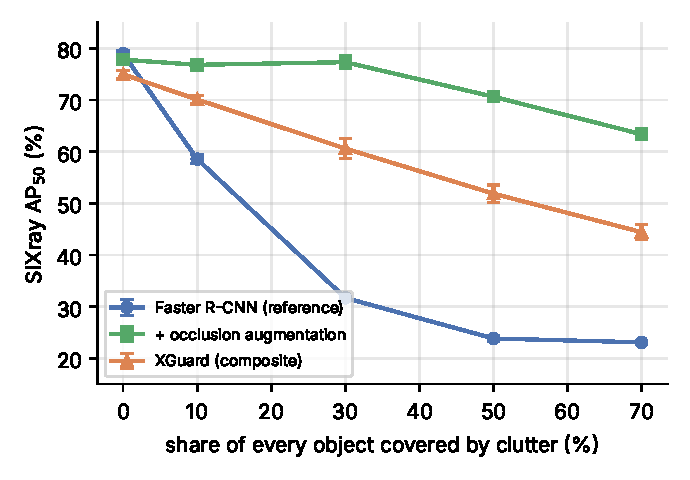
\includegraphics[width=0.92\linewidth]{figures/fig4_occlusion.pdf}
\caption{SIXray AP$_{50}$ as a growing share of every object is covered by clutter cut from other bags (mean $\pm$ SD over three seeds).}
\label{fig:occ}
\end{figure}

\paragraph{F4: Source-calibrated referral budgets do not transfer.} Thresholds that refer 10\% of SIXray validation bags refer between 2.9\% (risk head) and 51.6\% (energy score~\cite{liu2020energy}) of PIDray bags (\cref{tab:ref}). The missed-threat rate mostly follows how many bags are referred. Energy misses only 25.7\% of threats because it sends half of all bags to manual inspection, whereas MSP misses 62.7\% while referring 4.1\%. A score can be judged only at its realized operating point, and none of the scores keeps its operating point under shift.

\begin{table}[t]
\centering\small\setlength{\tabcolsep}{3pt}
\begin{tabular}{llcc}
\toprule
model & risk score & realized referral & missed threats $\downarrow$ \\
\midrule
\multirow{5}{*}{Reference} & MSP~\cite{hendrycks2017msp} & 4.1\pmm{0.7} & 62.7\pmm{1.3} \\
 & entropy & 13.9\pmm{0.5} & 58.7\pmm{1.0} \\
 & energy~\cite{liu2020energy} & 51.6\pmm{0.6} & 25.7\pmm{0.2} \\
 & unknown score & 9.4\pmm{1.0} & 60.6\pmm{0.7} \\
 & risk head & 2.9\pmm{0.1} & 62.9\pmm{1.1} \\
\midrule
\multirow{5}{*}{XGuard} & MSP & 10.0\pmm{3.0} & 61.8\pmm{2.5} \\
 & entropy & 28.6\pmm{7.4} & 48.8\pmm{5.4} \\
 & energy & 35.7\pmm{2.4} & 41.5\pmm{1.5} \\
 & unknown score & 1.9\pmm{0.3} & 67.8\pmm{0.3} \\
 & risk head & 24.5\pmm{7.9} & 51.6\pmm{5.5} \\
\bottomrule
\end{tabular}
\caption{Referral on PIDray (new scanner) at a nominal 10\% budget fixed on SIXray validation (\%, three seeds). The realized rate should be 10; deviations show that the operating point does not transfer.}
\label{tab:ref}
\end{table}

% -------------------------------------------------------------------------------------
\section{Diagnosing Remedies}
\label{sec:remedies}
\paragraph{A composite of representative remedies.} To test whether published ideas fix these failures, we add five modules to the same detector and call the result XGuard. Each module follows a common recipe: (a) a frequency-gated FPN adapter trained with \emph{scanner counterfactuals} (random attenuation curves, dual-energy color response, hue mapping, blur and sensor noise) and a feature-consistency loss; (b) reliability-weighted attention over RoI tokens with a consistency loss between clean and synthetically occluded views; (c) prototype classification from visual, CLIP~\cite{radford2021clip} text and attribute prototypes; (d) feature-space unknown synthesis that mixes factors of different known classes, in the spirit of VOS~\cite{du2022vos}, with a binary unknown head and an entropy loss; and (e) a learned risk head. The occluded views use clutter cut from other bags. Data, schedule and checkpoint selection are identical to the reference. As a control, we train the reference with the \emph{same} occlusion corruption as plain data augmentation (``+ occl.\ aug.'').

\paragraph{The simplest remedy wins.} Plain occlusion augmentation nearly removes the occlusion problem: AP$_{50}$ at 30\% coverage rises from 31.7 to 77.3, and the relative degradation falls from 0.71 to 0.19 (\cref{tab:occ,fig:occ}). It also helps on real data. It gains 2.6 AP$_{50}$ on the new scanner, 4.1 on PIDray's hidden subset, and doubles unseen-threat recall on hidden bags (9.3\% $\rightarrow$ 20.0\%). The cost is 1.1 AP$_{50}$ in-domain and more unknowns labeled as a known class on HiXray (AOSE 2.7 $\rightarrow$ 15.3). XGuard is more robust to occlusion than the reference, but less robust than the control at every coverage level. It is also worse everywhere else: $-$4.0 AP$_{50}$ in-domain and $-$6.1 on PIDray. Its occlusion gain is therefore explained by exposure to the corruption, not by the consistency machinery around it.

\paragraph{Scanner simulation does not transfer.} The adapter makes features almost invariant to the \emph{simulated} scanners: the cosine similarity between an object and its counterfactual rises from 0.925 to 0.996. Yet a linear probe identifies the real source dataset of an object \emph{more} easily (0.872 \vs 0.835), and PIDray AP$_{50}$ falls by 6.1 (seed-0 paired bootstrap: $-$5.8, 95\% CI $[-6.6,-5.2]$). Invariance to the simulator does not carry over to real scanner shift.

\paragraph{Outlier synthesis fails silently.} Feature-space synthesis is a standard way to give a closed-set detector an unknown score~\cite{du2022vos}. In our setting it collapses (\cref{tab:unk}). In all three seeds the unknown-head loss falls from 1.39 to 0.04--0.12 by the end of the first epoch and settles at 0.002, while the entropy term stays at its maximum ($1.61\approx\ln 5$) and gives no signal. The synthetic samples are trivially separable. Their mean maximum cosine similarity to the learned class prototypes is $-0.19$, against $+0.16$ for real training objects, and this similarity is itself an input of the unknown head. Separability is not the only problem, however. \cref{fig:shortcut} shows that real unseen PIDray objects are bimodal: most lie far from the known support (cosine $\approx$0.2 to the nearest SIXray class centroid), the rest lie on it ($\approx$1.0), and almost none fall in the narrow band (0.8--0.9) occupied by the synthetic samples. The far mode may partly reflect the scanner change, since the reference objects come from SIXray. Either way, the head is trained on a region where real unknowns rarely appear. The result is worse than having no unknown head. Unseen recall drops to 0.0\%, unknowns on HiXray are absorbed into known classes (AOSE 102.7 \vs 2.7), and the unknown score is \emph{inverted} (locAUROC 32.0). Replacing the synthesis by Gaussian noise around known embeddings prevents the collapse (final loss 0.80; synthetic and real similarities 0.11 \vs 0.12) and raises recall to 34.8\%, but the score is still inverted (locAUROC 27.6). Removing the shortcut is therefore not sufficient. Because the training loss looks excellent in the collapsed case, the failure is invisible without an open-world evaluation such as CoShift-X.

\begin{table}[t]
\centering\small\setlength{\tabcolsep}{2.6pt}
\resizebox{\columnwidth}{!}{%
\begin{tabular}{lcccc}
\toprule
unknown supervision & SIXray AP$_{50}$ & PIDray U-R$_{50}$ & PIDray locAUROC & final $\mathcal{L}_{unk}$ \\
\midrule
none (reference) & \ub{78.9}\pmm{0.6} & 11.4\pmm{1.7} & \ub{46.8}\pmm{2.0} & -- \\
Gaussian noise$^\ast$ & 72.7 & \ub{34.8} & 27.6 & 0.80 \\
factor mixing (XGuard) & 74.9\pmm{0.8} & 0.0\pmm{0.0} & 32.0\pmm{1.5} & 0.002 \\
\bottomrule
\end{tabular}}
\caption{Unknown supervision. locAUROC below 50 means the unknown score is inverted. $^\ast$One seed, 8 epochs, evaluated on a fixed 3{,}000-image PIDray subset; the other rows use three seeds, 12 epochs and the full test sets.}
\label{tab:unk}
\end{table}

\begin{figure*}[t]
\centering
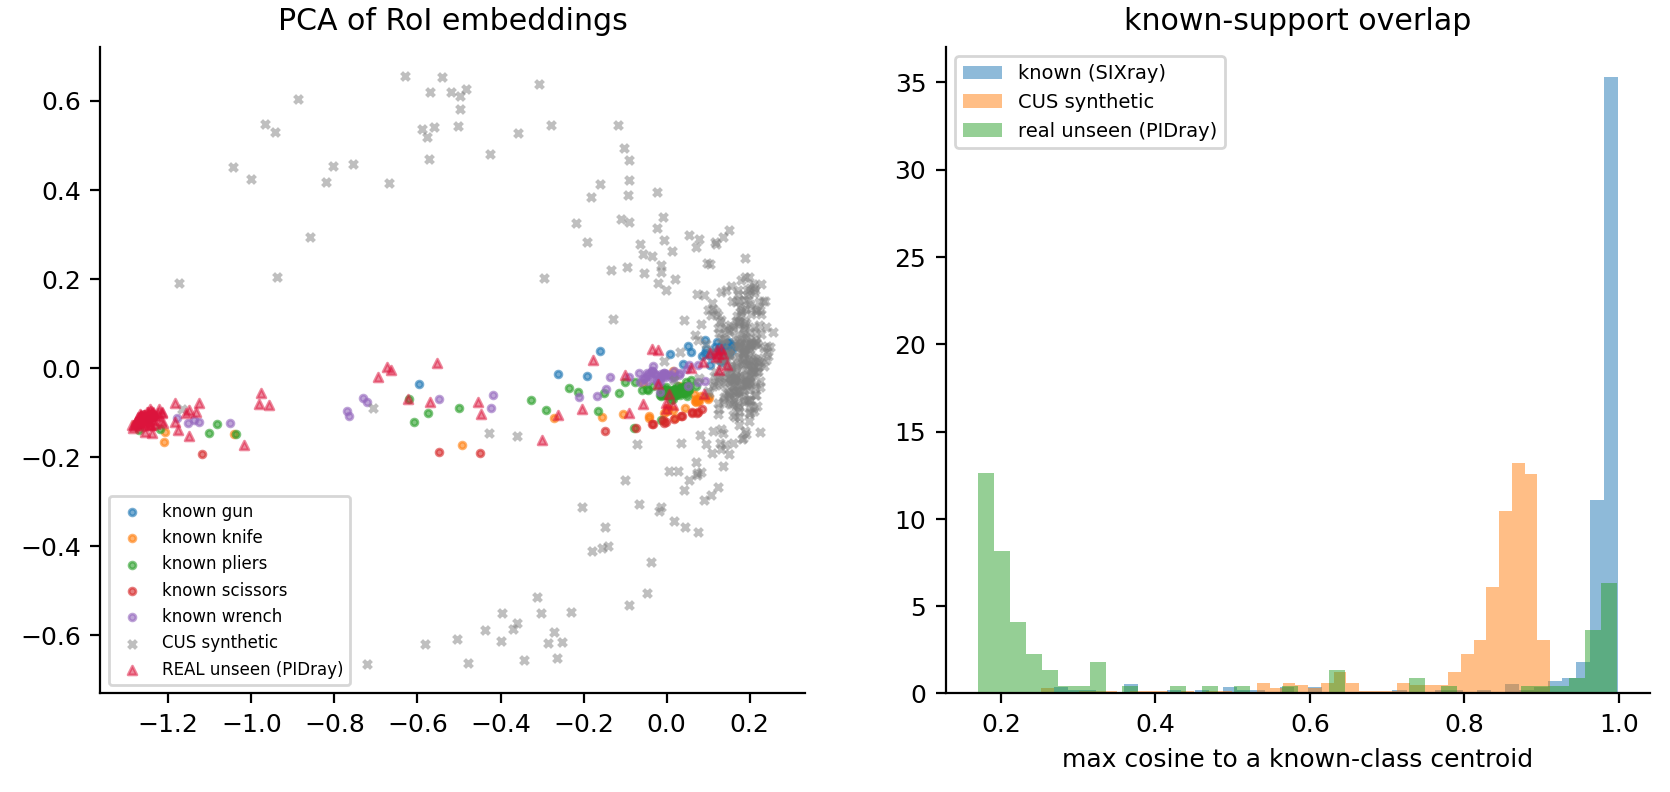
\includegraphics[width=0.78\textwidth]{figures/fig6_cus_validity.png}
\caption{Where synthetic unknowns lie. Left: PCA of RoI embeddings (XGuard). Right: maximum cosine similarity to a known-class centroid for known SIXray objects, synthetic unknowns and real unseen PIDray objects. Synthetic samples occupy a narrow band that real unknowns rarely enter.}
\label{fig:shortcut}
\end{figure*}

% -------------------------------------------------------------------------------------
\section{Discussion and Limitations}
\label{sec:discussion}
\textbf{Recommendations.} (1) Report exact, harmonized and hierarchical scores separately. (2) Audit lineage and duplicates before training on mirrors of public data. (3) Never report an unknown-detection method without localization AUROC on \emph{real} unknowns: a near-zero training loss can hide an inverted score. (4) Report referral at the \emph{realized} rate on the target, and recalibrate thresholds for each deployment site. (5) Before adding occlusion-specific modules, compare against the same corruption used as plain augmentation.

\textbf{Limitations.} (i) The SIXray source is a five-class mirror with a re-drawn split, because it is the only box-annotated public copy available to us. The three target datasets use their official splits, and we release lineage and split lists so that results can be re-run on the canonical split. (ii) All trained models share one two-stage architecture; we did not evaluate DETR-family or open-vocabulary detectors. (iii) We did not re-train the published open-world systems (ORE, OW-DETR, OpenDet, PROB); our unknown-supervision comparison covers feature-space synthesis and Gaussian noise in a shared detector, and the Gaussian variant uses one seed and a shorter schedule. (iv) The synthetic sweep is complemented by PIDray's real concealment subsets; OPIXray occlusion-level results require the official lists. (v) Occlusion augmentation increases open-set errors on HiXray, so it is not a free lunch for open-world detection.

\textbf{Use of LLMs.} An LLM-based coding assistant helped write experiment code and edit the text. The authors designed the study, ran all experiments, checked every reported number against the logged outputs, and take full responsibility for the content.

\section{Conclusion}
CoShift-X shows that X-ray threat detectors that look strong in-domain fail on new scanners, on unseen threats and under occlusion, and that the scores meant to flag these failures lose their operating point. A single occlusion augmentation outperforms a composite of five published remedies, while feature-space outlier synthesis is a trap that a closed-set evaluation cannot reveal. We hope that the benchmark, the audit lists and the evaluation code make these failures visible before deployment.

{\small
\bibliographystyle{ieeenat_fullname}
\bibliography{refs}
}
\end{document}
